% vim: spell spelllang=en:
\documentclass[12pt, oneside]{article}
\usepackage[a4paper, left=2.5cm, right=2.5cm, top=2.5cm, bottom=2.5cm]{geometry}

\usepackage[utf8]{inputenc} % Use unicode
\usepackage[T1]{fontenc}
\usepackage[english]{babel} % Names in spanish

%% Bibliography:
%\usepackage{comment}
%\usepackage[
    %backend=biber,
    %style=numeric,
%]{biblatex}
%\DeclareNameAlias{default}{last-first}

%\usepackage{csquotes}       % For bibliography quotations
%\DeclareQuoteAlias{spanish}{catalan}

%\addbibresource{biblio.bib}
%% see:
%% https://www.sharelatex.com/learn/Bibliography_management_in_LaTeX#The_bibliography_file

%\usepackage{datetime} % Customize date
%% \monthyeardate\today gives the date without the day
%\newdateformat{monthyeardate}{%
    %\monthname[\THEMONTH], \THEYEAR}

% For cross references
\usepackage[colorlinks = true]{hyperref}
\usepackage[catalan]{varioref}
%\usepackage{cleveref}
%hyperref configuration so that it doesn't contrast so much colorlinks,
\hypersetup{
   linkcolor={black},
   citecolor={black},
   %linkcolor={red!50!black},
   %citecolor={blue!50!black},
   urlcolor={blue!80!black}
}

\usepackage{xcolor}     % color

\usepackage{mathtools}  % amsmath + more
\usepackage{amsthm}     % Theorem enviroment
\usepackage{amssymb}    % More symbols
\usepackage{amstext}    % Text inside mathenv

\usepackage{relsize}    % Bigger math with mathlarger{___}
\usepackage{nicefrac}   % nice fractions in one line

\usepackage[export]{adjustbox}  % Adjust table size
\usepackage{float}              % Force tables and images position (H and H!)
\usepackage{wrapfig}            % Wrap images like in HTML

\usepackage{tabularx, colortbl, booktabs}    % Better tables
\usepackage{longtable}                      % Multiple page table

% Split cell in lines and more formating options inside table
\usepackage{array, multirow, multicol, makecell}

%\usepackage{subcaption}                     % Subfigures
%\usepackage[framemethod=tikz]{mdframed}     % Custom frames

%\usepackage[bottom]{footmisc} % Footnotes at bottom of page

%\usepackage[alsoload=hep]{siunitx}          % SI units and uncertainties
%\sisetup{locale = FR}                       % Commas and so on for spanish
%\sisetup{separate-uncertainty=true}
%\sisetup{
  %per-mode=fraction,
  %fraction-function=\nicefrac
%}

%\usepackage{tikz}
%%\usetikzlibrary{arrows}
%%\usetikzlibrary{scopes}
%\usetikzlibrary{babel}

%\usepackage{listings}       % For code blocks

%% Custom code highlight
%\definecolor{codegreen}{rgb}{0,0.6,0}
%\definecolor{codegray}{rgb}{0.5,0.5,0.5}
%\definecolor{codepurple}{rgb}{0.58,0,0.82}
%\definecolor{backcolour}{rgb}{0.95,0.95,0.92}
%\definecolor{lightblue}{RGB}{135,206,250}

%\lstdefinestyle{mystyle}{ backgroundcolor=\color{backcolour},
    %commentstyle=\color{codegreen}, keywordstyle=\color{blue},
    %numberstyle=\tiny\color{codegray}, stringstyle=\color{red},
    %identifierstyle=\color{black}, basicstyle=\footnotesize,
    %%breakatwhitespace=false,
    %breaklines=true,
    %%captionpos=b,                    keepspaces=true,
    %numbers=left,                    numbersep=5pt,
    %showspaces=false,
    %%showstringspaces=false, showtabs=false,
    %tabsize=4
%}
%\lstset{style=mystyle}

\newcommand{\whitepage}{
    \clearpage\thispagestyle{empty}\addtocounter{page}{-1} \newpage \clearpage
}

% Add command before appendix session for page numbering: A-1
%\newcommand{\appendixpagenumbering}{
    %\break
    %\pagenumbering{arabic}
    %\renewcommand{\thepage}{\thesection-\arabic{page}}
%}

%% Custom Math operators (functions not in italic in math mode):
%\DeclareMathOperator{\arcsec}{arcsec}
%\DeclareMathOperator{\arccot}{arccot}
%\DeclareMathOperator{\arccsc}{arccsc}
%\DeclareMathOperator{\cis}{cis}


\usepackage{caption}
\usepackage{subcaption}
\usepackage{graphicx}
\usepackage{enumitem}
\usepackage{lipsum}

\usepackage{siunitx}
\usepackage{hyphenat}

\usepackage{xcolor}

\definecolor{LightGray}{rgb}{0.83, 0.83, 0.83}
\definecolor{bg}{HTML}{282828}

\usepackage[newfloat]{minted}
\captionsetup[listing]{position=top}

\setminted{
style=monokai,
%frame=lines,
framesep=2mm,
baselinestretch=1.2,
breaklines,
bgcolor=bg,
fontsize=\footnotesize,
linenos
}

\renewcommand\theadfont{\bfseries}

\title{
    PAR Laboratory Assignment\\
    Lab 3: Embarrassingly parallelism with OpenMP:\\ Mandelbrot set
}

\author{
    par2109:
    Aleix Boné,
    Alex Herrero
}

\date{
    Spring 2019-20
}

\begin{document}

\thispagestyle{empty}
\clearpage
\setcounter{page}{-1}

\begin{titlepage}
{
    \centering
    \null
    \vfill
    {\Huge \bfseries PAR Laboratory Assignment\par}
    \vspace{3em}
    {\Large {\scshape Lab 3:} Embarrassingly parallelism with OpenMP: \\ Mandelbrot set \par}
    \vfill
\begin{center}
\end{center}
    \vspace{3cm}

    \vfill
    {\raggedleft \Large
        Aleix Boné\\
        Alex Herrero\\
        {\bfseries\ttfamily par2109}\\
        \vspace{4em}
        2020-04-16
        \par}
}
\end{titlepage}

\tableofcontents
\pagebreak


\section{Introduction}%
\label{sec:Introduction}

% copy paste form here to ... 
% (solo he cambbiado el tiempo verbal, no se si hace falta cambiarlo más ya que enrealidad lo que queremos decir al principio es lo mismo que dice el enunciado...) (y bueno he borrado un par de parrafos)
In this laboratory assignment we explored the tasking model in OpenMP to express iterative task decompositions. 
We started by exploring the most appropriate ones by using \emph{Tareador}. The program that we used is the computation of the \emph{Mandelbrot set}, a particular set of points, in the complex domain, whose boundary generates a distinctive and easily recognisable two-dimensional fractal shape.

For each point $c$ in a delimited two-dimensional space, the complex quadratic polynomial recurrence $z_{n+1} = z^2_n + c$ is iteratively applied in order to determine if it belongs or not to the Mandelbrot set.  The point is part of the Mandelbrot set if, when starting with $z_0 = 0$ and applying the iteration repeatedly, the absolute value of $z_n$ never exceeds a certain number however large $n$ gets.

We analyzed the potential parallelism for two possible task granularities that can be exploited in this program. Those two are:
\begin{enumerate}[label=\alph*)]
\item \emph{Point}: a task corresponds with the computation of a single point (\texttt{row},\texttt{col}) of the Mandelbrot set.
\item \emph{Row}: a task corresponds with the computation of a whole \texttt{row} of the Mandelbrot set.
\end{enumerate}
% ... here

We executed both, \texttt{mandel-tar}\footnote{\texttt{mandel}: used for timing purposes and to check for the numerical validity of the output (non-graphical version).} and \texttt{mandeld-tar}\footnote{\texttt{mandeld}: generates a binary that visualizes the Mandelbrot set (graphical version).}, programs with the different granularities using the \texttt{./run-tareador.sh} script and we obtained the following results.

\begin{figure}[H]
\centering

\includegraphics[width=\textwidth]{plots/dependency_graph_mandel_point.png}
\caption{Task dependence graph of \texttt{mandel-tar.c} with point decomposition.}
\label{graph:mandel_point}
\end{figure}

\begin{figure}[H]
\centering
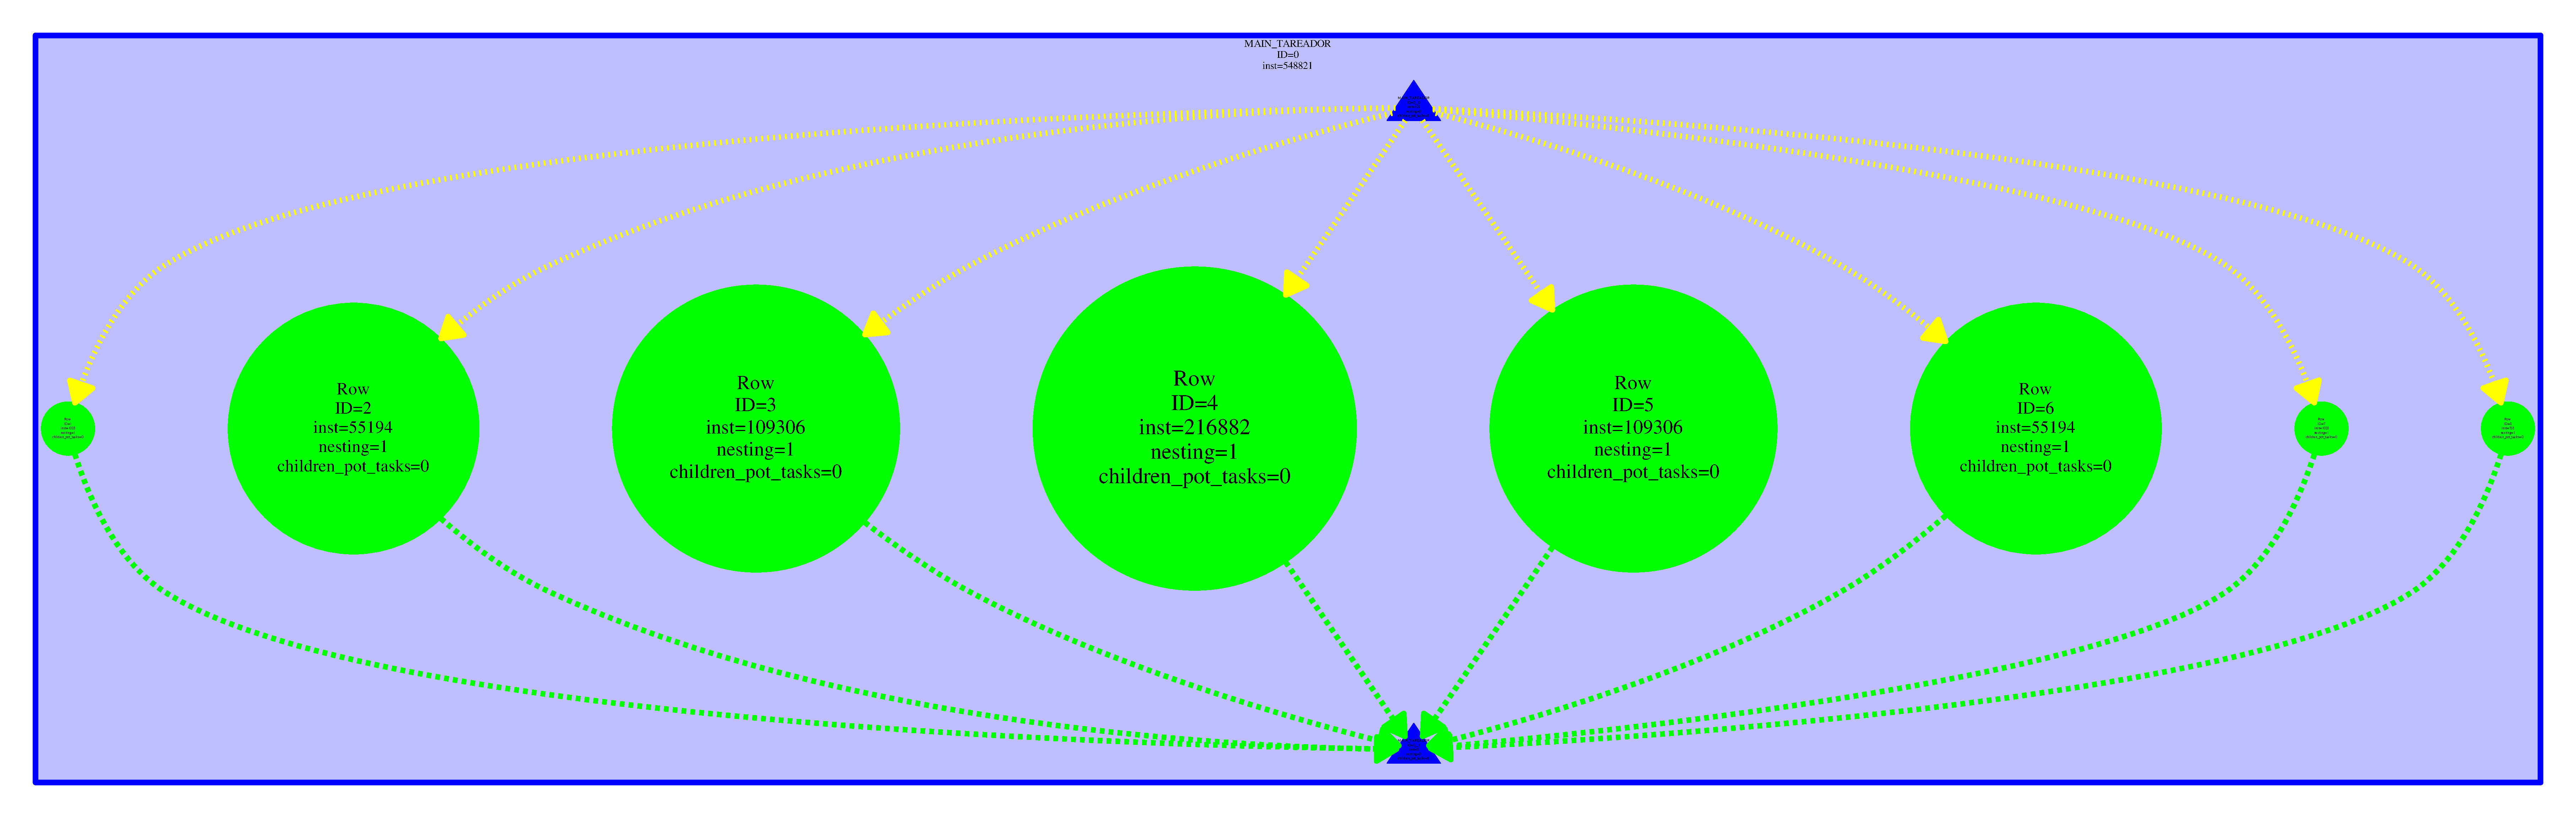
\includegraphics[width=0.6\textwidth]{plots/dependency_graph_mandel_row.pdf}
\caption{Task dependence graph of \texttt{mandel-tar.c} with row decomposition.}
\label{graph:mandel_row}
\end{figure}

% Which are the two most important common characteristics of the task graphs generated for the two task granularities (Point and Row) for the non-graphical version of mandel-tar?  Why the task graphs generated for mandel-tar and mandeld-tar are so different?  Which section of the code do you think is causing the serialization of all tasks in the graphical version?  How will you protect this section of code in the parallel OpenMP code in the next sections?

As we expected the point decomposition has a much more big granularity than the row one. But we obtained that the two decompositions generate similar task graphs for each executable.

We can observe in figures~\ref{graph:mandel_point} and~\ref{graph:mandel_row} that with the \texttt{mandel} executable all tasks can parallelize at the same level. But in figure~\ref{graph:mandeld_point_and_row} we see that with the \texttt{mandeld} executable we obtain a serialization of all tasks.

\begin{figure}[H]
\centering

\includegraphics[height=8cm]{plots/dependency_graph_mandeld_point.png}
\hspace{5em}
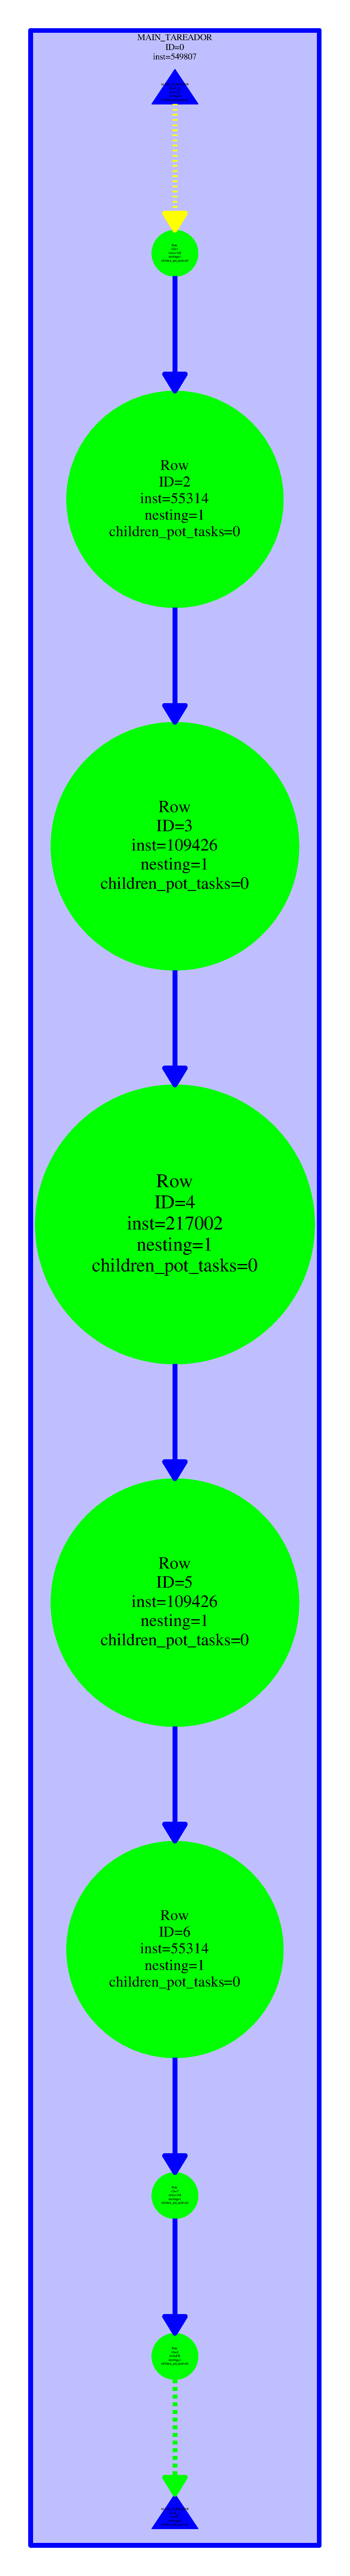
\includegraphics[height=8cm]{plots/dependency_graph_mandeld_row.pdf}
\caption{Task dependence graph of \texttt{mandeld-tar.c} with point and row decompositions.}
\label{graph:mandeld_point_and_row}
\end{figure}

This serialization in the graphical version is caused in the lines 120-130 of the code due to a data race when accessing the display, this implies full dependence between all tasks. Therefore when parallelizing the program with OpenMP, this section has to be protected with the \texttt{\#pragma omp critical} clause as shown in the listing~\ref{listing:mandel-omp-critical}.

\begin{listing}[H]
\inputminted[firstline=120,lastline=130]{c}{sources/mandel-omp-v1.c}
\caption{Problematic section in \texttt{mandel-omp.c} protected with \texttt{\#pragma omp critical}.}
\label{listing:mandel-omp-critical}
\end{listing}

% Reason which one of the two task granularities would be more appropriate to apply to implement a parallel version of the Mandelbrot code.

The program is embarrassingly parallelizable so to implement a parallel version of the Mandelbrot code the point granularity should be more appropriate. But with a low number of threads the overhead of task creation would increase and in that case the row granularity could have a better final execution time.

We can also see that there is a big variation in the number of instructions per task, specially in the point decomposition.
This is due to the recursive nature of the mandelbrot set computation, where we can't know how many iterations it'll
take to compute each point. The problematic loop is shown in listing~\ref{listing:mandel-omp-dowhile} where we can see
that for each point it could take from 1 to \texttt{maxiter} iterations of the loop to compute.

\begin{listing}[H]
\inputminted[firstline=109,lastline=118]{c}{sources/mandel-omp-v1.c}
\caption{Problematic section in \texttt{mandel-omp.c}}
\label{listing:mandel-omp-dowhile}
\end{listing}

\section{Parallelization Strategies}%
\label{sec:Parallelization Strategies}

%TODO: aqui explicas las strategias del 4.2, 4.3 y 4.4

\subsection{\emph{Point} startegy using \emph{OpenMP} \texttt{task}}%

There are multiple ways to create a task for the computation of each point in the Mandelbrot set. We tried
several options and analyzed the performance of each one.

The first version is shown in listing~\ref{lst:v1}. We create a task for each iteration of the \texttt{col} for. The
pool of threads is initialized at every row.

\begin{listing}[H]
    \caption{v1 of point task decomposition}
    \inputminted[firstline=91,lastline=98]{c}{sources/mandel-omp-v1.c}
    \label{lst:v1} 
\end{listing}

In the second version we mode the parallel and single pragmas outside of the \texttt{row} loop. Therefore, there
is only one parallel region in the program. Since we also add a taskwait, the program should behave the same as with
version 1. 

\begin{listing}[H]
    \centering
    \caption{v2: point task decomposition with taskwait}
    \inputminted[firstline=91,lastline=98]{c}{sources/mandel-omp-v2.c}
    \vspace{-2em}
    \inputminted[firstline=132,lastline=134]{c}{sources/mandel-omp-v2.c}
    \label{lst:v2} 
\end{listing}

In v3 we use \texttt{taskgroup} instead of \texttt{taskwait}. The main diference between \texttt{taskgroup}
and \texttt{taskwait} is that the former waits for all tasks inside the group, including children tasks.
\texttt{taskwait} only waits for the tasks generated on the same level, and not the children of those tasks.
In our particular case, since there are no nested tasks generated, there should be no noticeable 
difference between v2 and v3.

\begin{listing}[H]
    \centering
    \caption{v3: point task decomposition with taskgroup}
    \inputminted[firstline=91,lastline=98]{c}{sources/mandel-omp-v3.c}
    \vspace{-2em}
    \inputminted[firstline=133,lastline=135]{c}{sources/mandel-omp-v3.c}
    \label{lst:v3} 
\end{listing}

v4 removes the \texttt{taskwait} directive, since there is no need to wait for the previous row tasks
to finish before generating the new ones.

\begin{listing}[H]
    \centering
    \caption{v4: point task decomposition task without taskwait}
    \inputminted[firstline=91,lastline=98]{c}{sources/mandel-omp-v4.c}
    \vspace{-2em}
    \inputminted[firstline=131,lastline=133]{c}{sources/mandel-omp-v4.c}
    \label{lst:v4} 
\end{listing}

v5 uses \texttt{taskloop} to explicitly generate the tasks. Since there is no granularity, OpenMP
decides a value for it depending of the number of threads in the region.

\begin{listing}[H]
    \centering
    \caption{v5: point task decomposition with taskloop}
    \inputminted[firstline=91,lastline=98]{c}{sources/mandel-omp-v5.c}
    \label{lst:v5} 
\end{listing}

In v6 we specify a granularity of 1, meaning that every iteration loop is assigned to a single task

\begin{listing}[H]
    \centering
    \caption{v6: point task decomposition with taskloop grainsize(1)}
    \inputminted[firstline=91,lastline=98]{c}{sources/mandel-omp-v6.c}
    \label{lst:v6} 
\end{listing}

In v7 we specify a granularity of 1 and \texttt{nogroup} that eliminates the implicit \texttt{taskwait}
of the loop (meaning that they don't wait for the other tasks to finish before creating the next set).

\begin{listing}[H]
    \centering
    \caption{v7: point task decomposition with taskloop grainsize(1) nogroup}
    \inputminted[firstline=91,lastline=98]{c}{sources/mandel-omp-v7.c}
    \label{lst:v7} 
\end{listing}

\subsection{\emph{Row} startegy using \emph{OpenMP} \texttt{task}}%

To implement the \emph{row} parallelization strategy we defined a task for each iteration of
the \texttt{row} loop as shown in listing~\ref{lst:v8}.

\begin{listing}[H]
    \centering
    \caption{v8: row task decomposition}
    \inputminted[firstline=91,lastline=98]{c}{sources/mandel-omp-v8.c}
    \label{lst:v8} 
\end{listing}

\subsection{\texttt{for}-based parallelization}%

We used \texttt{\#pragma omp parallel for collapse(2)} to collapse the two levels of the for loops.

\begin{listing}[H]
    \centering
    \caption{for-based task decomposition}
    \inputminted[firstline=91,lastline=96]{c}{sources/mandel-omp-v11.c}
    \label{lst:v11} 
\end{listing}

%$ OMP_NUM_THREADS=1 ./mandeld-omp -i 10000
%Total execution time: 3.228077s
%$ ./mandeld -i 10000
%Total execution time: 3.061886s
%$ OMP_NUM_THREADS=8 ./mandeld-omp -i 10000
%Total execution time: 1.210712s

\section{Performance evaluation}%
\label{sec:Performance evaluation}

%TODO: Aqui comparas


\begin{figure}[H]
    \begin{minipage}{0.5\textwidth}
        \centering
        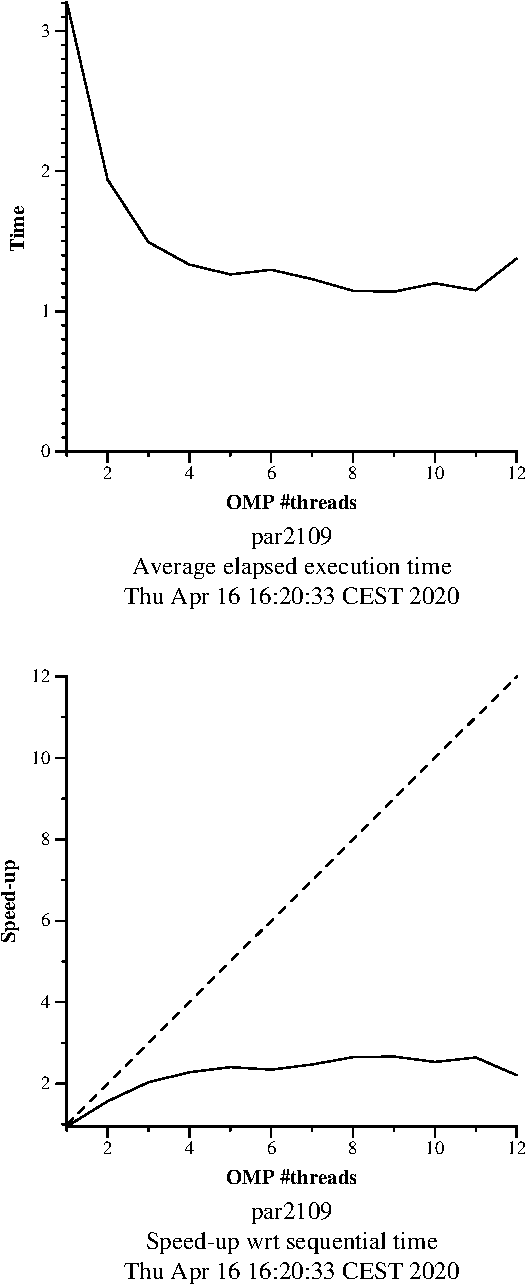
\includegraphics[width=0.7\linewidth]{plots/v1-crop.pdf}
        \caption{Strong scalability analysis v1}
        \label{fig:ssa_v1} 
    \end{minipage}
    \begin{minipage}{0.5\textwidth}
        \centering
        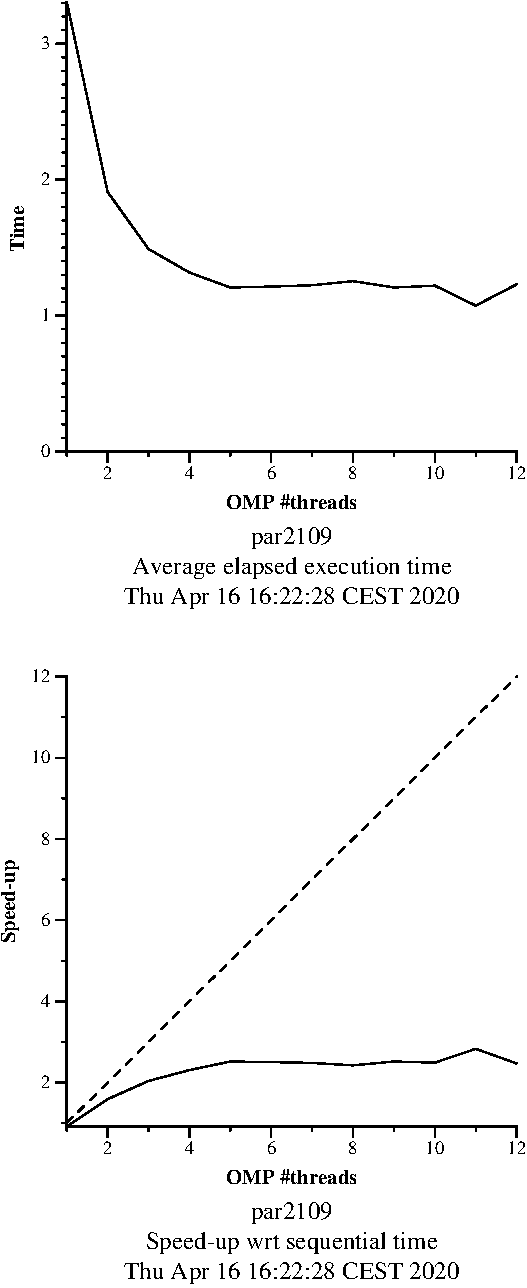
\includegraphics[width=0.7\linewidth]{plots/v2-crop.pdf}
        \caption{Strong scalability analysis v2}
        \label{fig:ssa_v2} 
    \end{minipage}
\end{figure}

\begin{figure}[H]
    \begin{minipage}{0.5\textwidth}
        \centering
        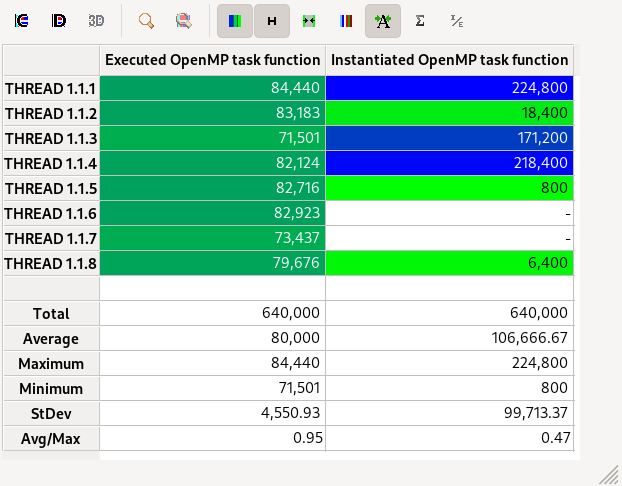
\includegraphics[width=0.7\linewidth]{captures/v1-profile.png}
        \caption{Paraver \texttt{tasks\_profile} v1}
        \label{fig:profile_v1} 
    \end{minipage}
    \begin{minipage}{0.5\textwidth}
        \centering
        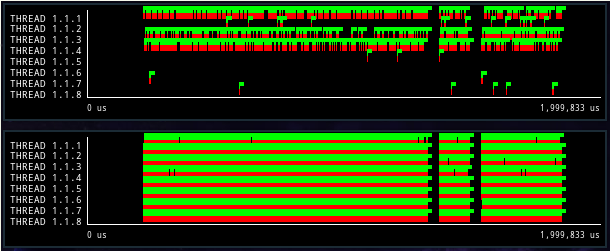
\includegraphics[width=\linewidth]{captures/v1-plot.png}
        \caption{Paraver tasks v1}
        \label{fig:tasks_v1} 
    \end{minipage}
\end{figure}

\begin{figure}[H]
    \begin{minipage}{0.5\textwidth}
        \centering
        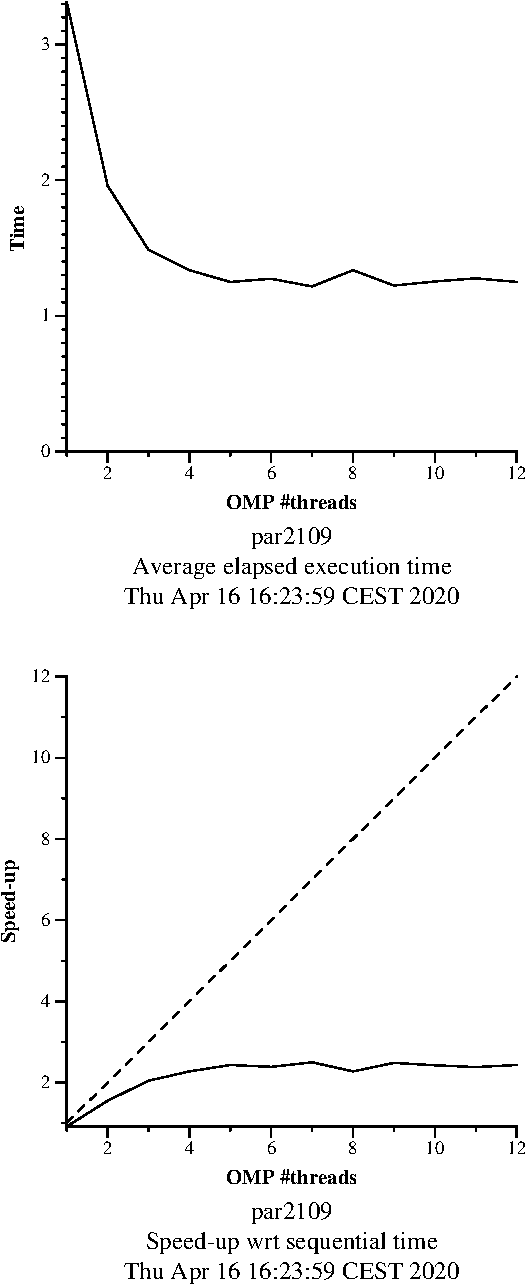
\includegraphics[width=0.7\linewidth]{plots/v3-crop.pdf}
        \caption{Strong scalability analysis v3}
        \label{fig:ssa_v3} 
    \end{minipage}
    \begin{minipage}{0.5\textwidth}
        \centering
        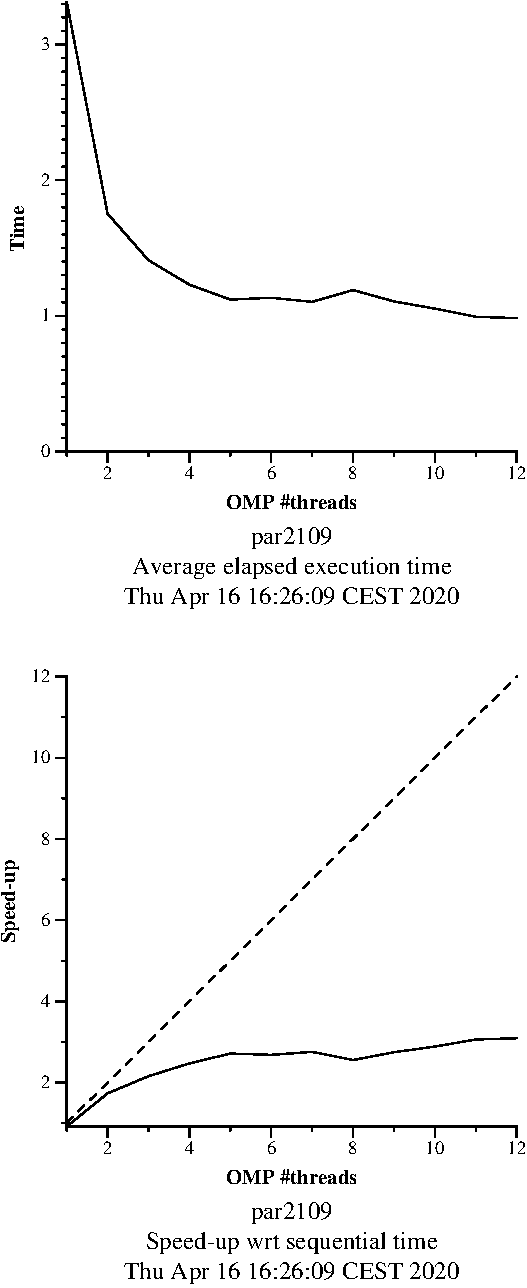
\includegraphics[width=0.7\linewidth]{plots/v4-crop.pdf}
        \caption{Strong scalability analysis v4}
        \label{fig:ssa_v4} 
    \end{minipage}
\end{figure}


\begin{figure}[H]
    \begin{minipage}{0.5\textwidth}
        \centering
        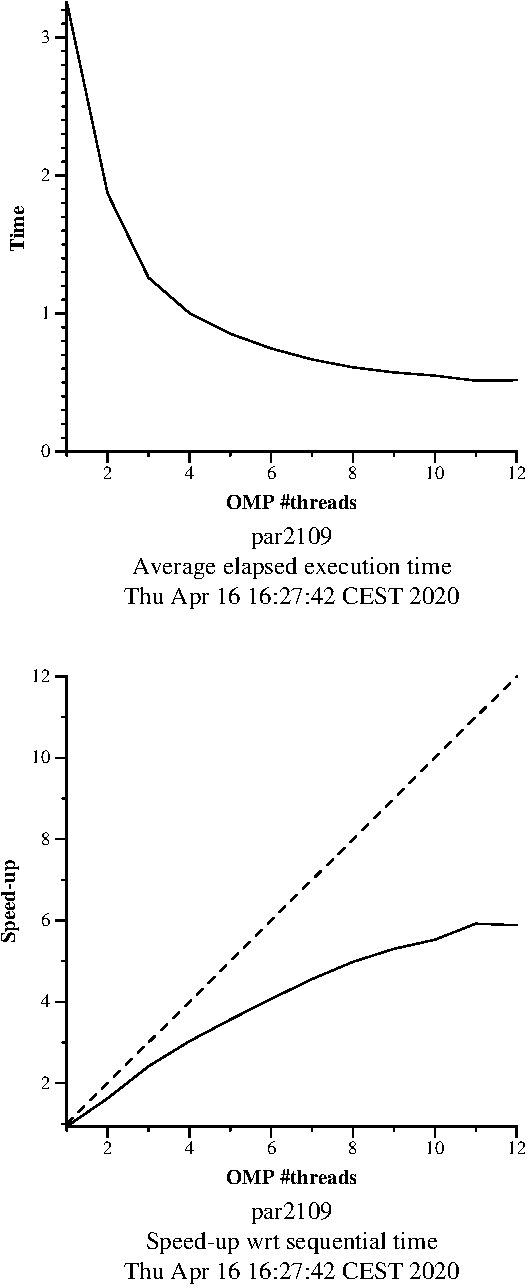
\includegraphics[width=0.7\linewidth]{plots/v5-crop.pdf}
        \caption{Strong scalability analysis v5}
        \label{fig:ssa_v5} 
    \end{minipage}
    \begin{minipage}{0.5\textwidth}
        \centering
        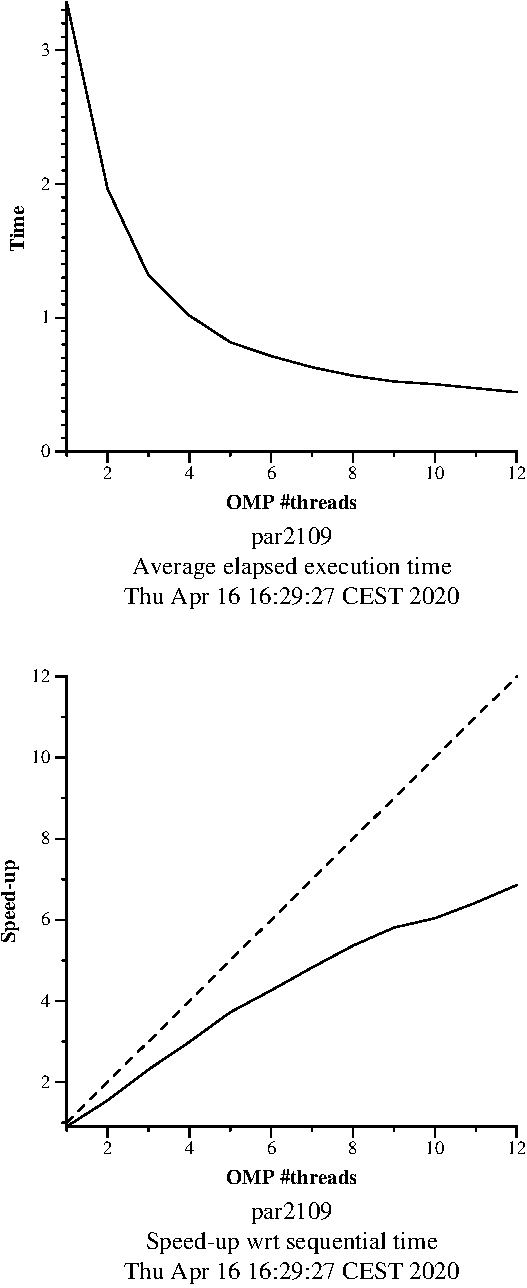
\includegraphics[width=0.7\linewidth]{plots/v6-crop.pdf}
        \caption{Strong scalability analysis v6}
        \label{fig:ssa_v6} 
    \end{minipage}
\end{figure}

\begin{figure}[H]
    \begin{minipage}{0.5\textwidth}
        \centering
        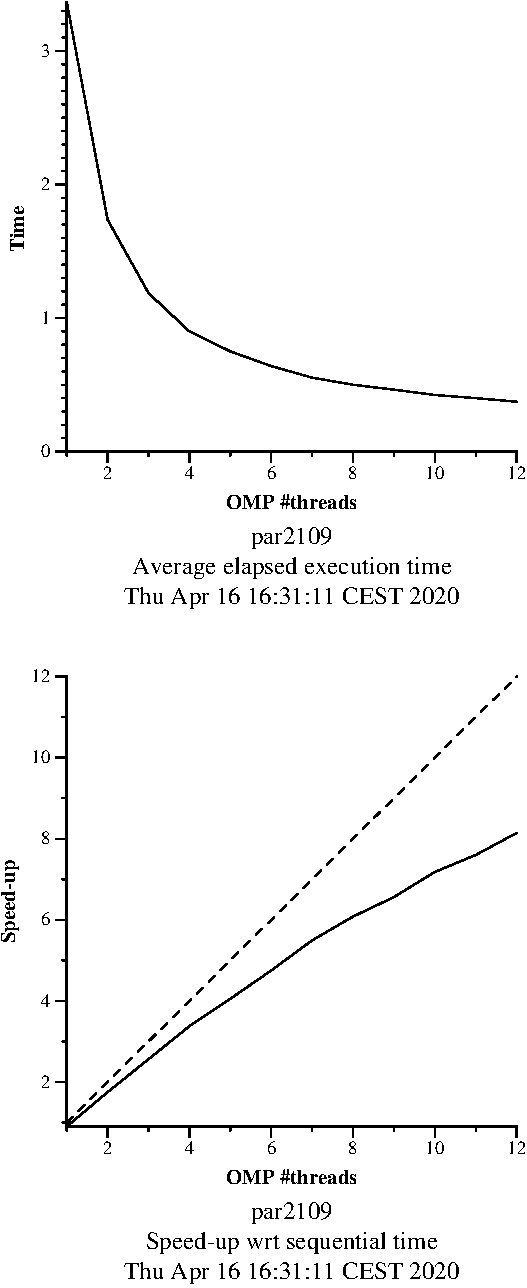
\includegraphics[width=0.7\linewidth]{plots/v7-crop.pdf}
        \caption{Strong scalability analysis v7}
        \label{fig:ssa_v7} 
    \end{minipage}
    \begin{minipage}{0.5\textwidth}
        \centering
        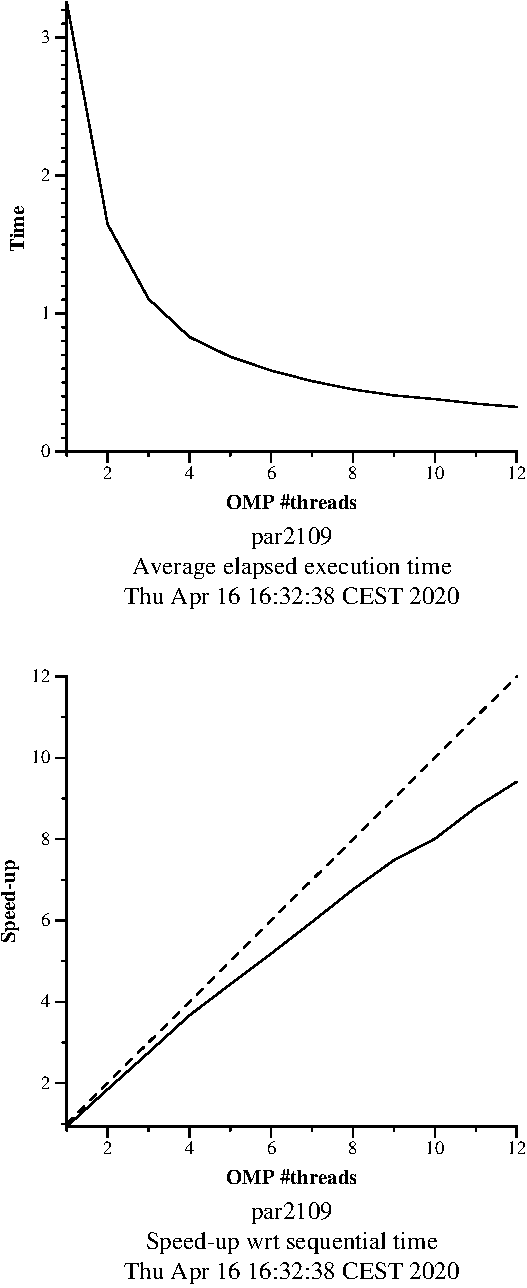
\includegraphics[width=0.7\linewidth]{plots/v8-crop.pdf}
        \caption{Strong scalability analysis v8}
        \label{fig:ssa_v8} 
    \end{minipage}
\end{figure}

\subsection{Taskloop grainsize analysis}

\begin{table}[H]
    \caption{Execution times with different grainsizes}%
    \label{tab:grainsize}
    \begin{center}
    \begin{tabular}{lr}
\toprule
{} &      time \\
grainsize &           \\
\midrule
1         &  0.317474 \\
2         &  0.361412 \\
5         &  0.372336 \\
10        &  0.256939 \\
25        &  0.208336 \\
50        &  0.196701 \\
100       &  0.183566 \\
200       &  0.181784 \\
400       &  0.185489 \\
800       &  0.185322 \\
\bottomrule
\end{tabular}

    \end{center}
\end{table}

\begin{figure}[H]
    \centering
    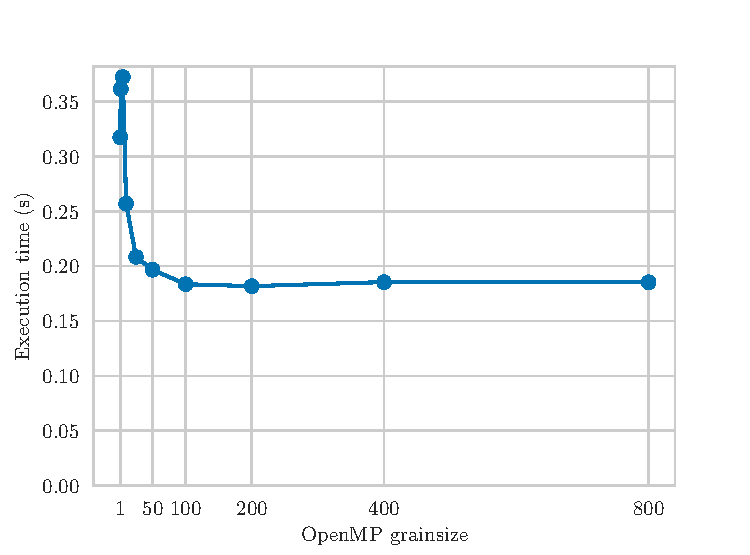
\includegraphics{plots/grainsize.pdf}
    \caption{Plot of execution time for different grainsizes}
    \label{fig:grain} 
\end{figure}

\begin{figure}[H]
    \centering
    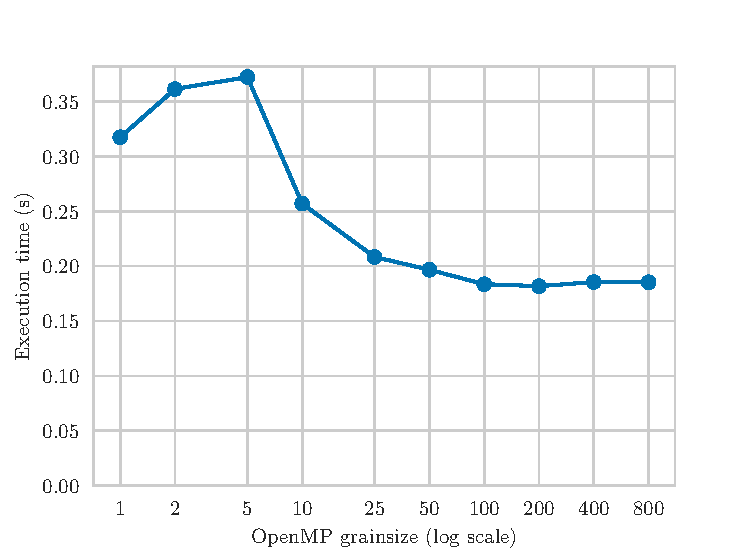
\includegraphics{plots/grainsize_log.pdf}
    \caption{Plot of execution time for different grainsizes (log scale)}
    \label{fig:grain_log} 
\end{figure}

\subsection{for scheduling analysis}

We ran the for task decomposition of the program with different scheduling schemes and chunk-sizes. The
results obtained can be seen in table~\ref{tab:for}.

\begin{table}[H]
    \caption{Execution times with different scheduling and chunk-sizes}%
    \label{tab:for}
    \begin{center}
    \begin{tabular}{llrrr}
\toprule
     & scheduling &   dynamic &    guided &    static \\
{} & chunk-size &           &           &           \\
\midrule
time & 1   &  0.198096 &  0.221012 &  0.186173 \\
     & 2   &  0.191246 &  0.220252 &  0.185386 \\
     & 5   &  0.186887 &  0.222712 &  0.201038 \\
     & 10  &  0.185859 &  0.222406 &  0.230312 \\
     & 25  &  0.185232 &  0.220492 &  0.234002 \\
     & 50  &  0.186607 &  0.219147 &  0.341946 \\
     & 100 &  0.187840 &  0.222233 &  0.557168 \\
     & 200 &  0.185515 &  0.220431 &  0.416928 \\
     & 400 &  0.189663 &  0.221099 &  0.256937 \\
     & 800 &  0.187154 &  0.219909 &  0.183334 \\
\bottomrule
\end{tabular}

    \end{center}
\end{table}

Figures~\ref{fig:for} and \ref{fig:for_log} show the data of table~\ref{tab:for} on a linear scale and logarithmic
scale respectively. We can see that chunk-size does not affect execution time with dynamic or guided scheduling
and that it severely affects the execution time with static scheduling. Guided scheduling provides no benefits, which
makes sense given that all tasks have the same cost. The best results are obtained with static scheduling and
a chunk size of 800, although similar execution times are obtained with static 1, 2 and dynamic scheduling.


\begin{figure}[H]
    \centering
    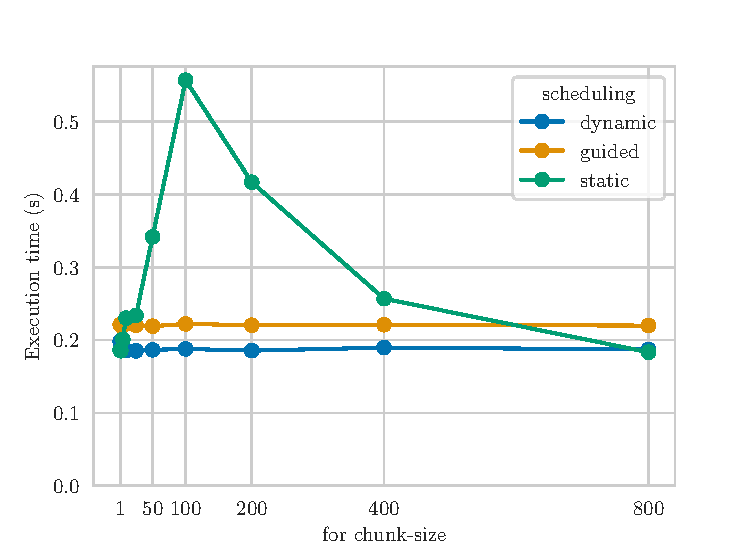
\includegraphics{plots/for-scheduling.pdf}
    \caption{Plot of execution time for different chunk-sizes and scheduling}
    \label{fig:for} 
\end{figure}

\begin{figure}[H]
    \centering
    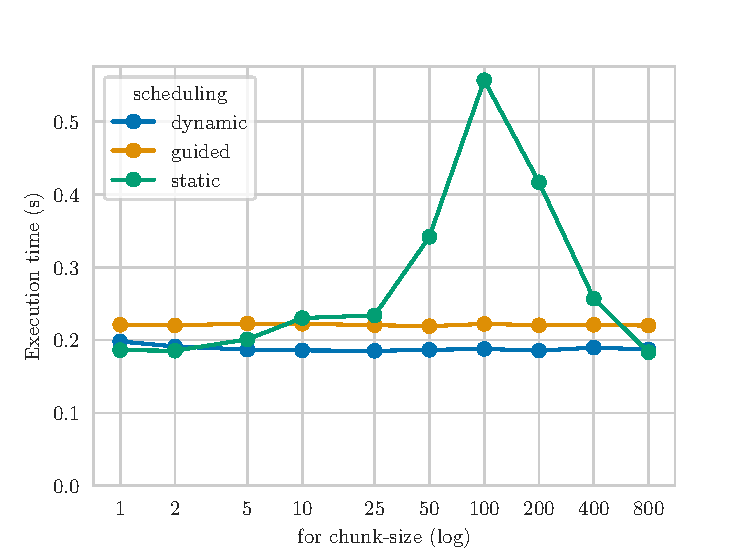
\includegraphics{plots/for-scheduling_log.pdf}
    \caption{Plot of execution time for different chunk-sizes and scheduling (log scale)}
    \label{fig:for_log} 
\end{figure}

The fact that static scheduling has much longer execution times for certain-chunk sizes is due to the load imbalance
we discussed in the introduction. One thing to notice is that the computation of a point takes longer in the \emph{edges}
of the set

\begin{figure}[H]
    \centering
    
\includegraphics{images/set.png}
    \caption{Mandelbrot set with 10000 maxiter}
    \label{fig:set} 
\end{figure}

\section{Conclusions}%
\label{sec:Conclusions}

% TODO: I aqui pues relleno bonito del final


\end{document}
